\documentclass[uplatex]{jsarticle}
\usepackage{listings, plistings, amsfonts, bm, amsmath, amssymb}
\usepackage[dvipdfmx]{graphicx}
\lstset{
  basicstyle={\ttfamily},
  identifierstyle={\small},
  commentstyle={\smallitshape},
  keywordstyle={\small\bfseries},
  ndkeywordstyle={\small},
  stringstyle={\small\ttfamily},
  frame={tb},
  breaklines=true,
  columns=[l]{fullflexible},
  numbers=left,
  xrightmargin=0zw,
  xleftmargin=3zw,
  numberstyle={\scriptsize},
  stepnumber=1,
  numbersep=1zw,
  lineskip=-0.5ex,
}
\parindent = 0pt

\title{2016年 解答}
\begin{document}
\section*{第1問}
\subsection*{(1)}

$
A =
\begin{pmatrix}
	1 & 1 & 1 \\
	1 & 0 & 0 \\
	0 & 1 & 0 \\
\end{pmatrix} $

\subsection*{(2)}
行基本変形を行うと,
$
\begin{pmatrix}
	1 & 1 & 1 \\
	1 & 0 & 0 \\
	0 & 1 & 0 \\
\end{pmatrix}
\rightarrow\begin{pmatrix}
	1 & 1 & 1 \\
	0 & -1 & -1 \\
	0 & 1 & 0 \\
\end{pmatrix}
\rightarrow\begin{pmatrix}
	1 & 1 & 1 \\
	0 & -1 & -1 \\
	0 & 0 & -1 \\
\end{pmatrix}
$
となるので,\underline{$rank(A) = 3$}. .\\
$E$を単位行列,$\lambda$を固有値とすると$|A-\lambda E| = 0$を満たし,これを計算することにより,\underline{$\lambda^3 - \lambda^2 - \lambda - 1 = 0$}を得る.

\subsection*{(3)}
$A^\prime = A-\lambda E = 
\begin{pmatrix}
	1-\lambda & 1 & 1 \\
	1 & -\lambda & 0 \\
	0 & 1 & -\lambda \\
\end{pmatrix}
$
とおく.$A^\prime$において,行基本変形を行うと,
$
\begin{pmatrix},
	0 & 1+\lambda(1-\lambda) & 1 \\
	1 & -\lambda & 0 \\
	0 & 1 & -\lambda \\
\end{pmatrix}
\rightarrow
\begin{pmatrix}
	1 & -\lambda & 0 \\
	0 & 1+\lambda(1-\lambda) & 1 \\
	0 & 1 & -\lambda \\
\end{pmatrix}
\rightarrow
\begin{pmatrix}
	1 & -\lambda & 0 \\
	0 & 1+\lambda(1-\lambda) & 1 \\
	0 & 1+\lambda+\lambda(1-\lambda) & 0 \\
\end{pmatrix}
$
となる.\\
よって,固有値$\lambda_k,(k=1, 2, 3)$に対応する固有ベクトルを$\begin{pmatrix}x_k & y_k & z_k\end{pmatrix}^T$とおくと,
$$
\begin{cases}
	x_k - \lambda y_k = 0 \\
	(1 + \lambda - \lambda^2)y_k + z_k = 0
\end{cases}
$$
を満たすので,固有ベクトルの1つは
\underline{
$
\begin{pmatrix}\lambda_k & 1 & \lambda_k^2-\lambda_k-1\end{pmatrix}^T
$
}
となる.

\subsection*{(4)}
$f(\lambda) = \lambda^3 - \lambda^2 - \lambda - 1$とおく.\\
$f^\prime(\lambda) = 3\lambda^2-2\lambda-1 = (\lambda-1)(3\lambda-1)$.\\
以上より,増減表は以下のようになる.
\begin{table}[htb]
	\begin{tabular}{|c|c c c c c|}\hline
		$\lambda$ & ... & $-\frac{1}{3}$ & ... & 1 & ... \\ \hline
		$f^\prime$ & + & 極大 & - & 極小 & + \\ \hline
		$f$ & $\nearrow$ & $-\frac{22}{27}$ & $\searrow$ & $-2$ & $\nearrow$ \\ \hline
	\end{tabular}
\end{table}
\\
よってグラフは \\
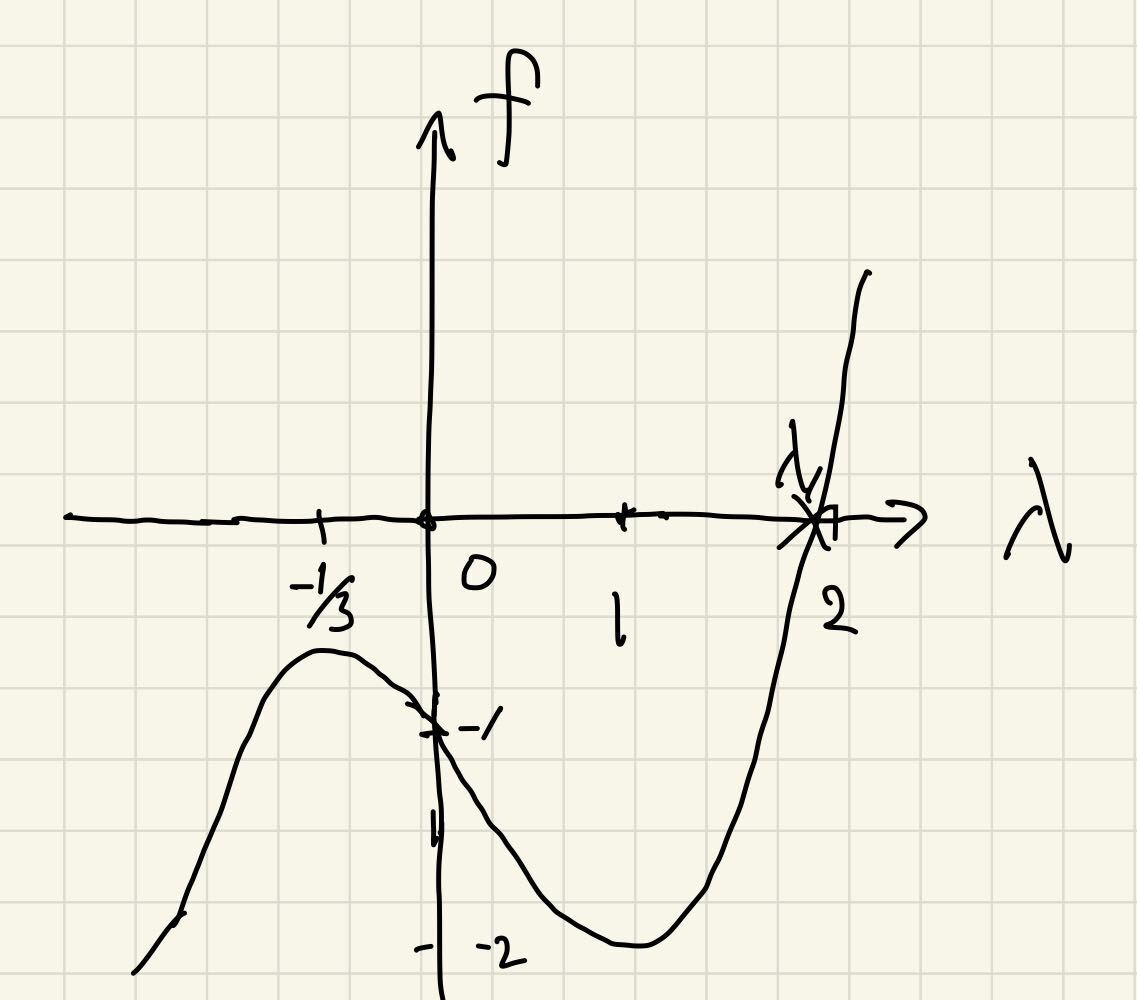
\includegraphics[width=50mm]{figure1.jpg}
となり,$\lambda$軸との交点はただ1つで,かつその交点$\lambda_1$は$1<\lambda_1<2$なので,題意は示された.(証明終)

\subsection*{(5)}
行列$A$は,正方行列
$P=
\begin{pmatrix}
	\lambda_1 & \lambda_2 & \lambda_3 \\
	1 & 1 & 1 \\
	\lambda_1^2-\lambda_1-1 & \lambda_2^2-\lambda_2-1 & \lambda_3^2-\lambda_3-1 \\
\end{pmatrix}
$
を用いて,\\
$P^{-1}AP =
\begin{pmatrix}
	\lambda_1 & 0 & 0 \\
	0 & \lambda_2 & 0 \\
	0 & 0 & \lambda_3 \\
\end{pmatrix} 
$
と対角化できる.
よって,
$\begin{pmatrix}
	\lambda_1^n & 0 & 0 \\
	0 & \lambda_2^n & 0 \\
	0 & 0 & \lambda_3^n \\
\end{pmatrix}
=P^{-1}A^nP$が成り立ち,
$
A^n=
P
\begin{pmatrix}
	\lambda_1^n & 0 & 0 \\
	0 & \lambda_2^n & 0 \\
	0 & 0 & \lambda_3^n \\
\end{pmatrix}
P^{-1}
$が成り立つ.\\
また,(1.1)より,
$$
\begin{pmatrix}
	T_{n+2} \\
	T_{n+1} \\
	T_{n} \\
\end{pmatrix}
= A^n
\begin{pmatrix}
	T_2 \\
	T_1 \\
	T_0 \\
\end{pmatrix}
=
\begin{pmatrix}
	\lambda_1 & \lambda_2 & \lambda_3 \\
	1 & 1 & 1 \\
	\lambda_1^2-\lambda_1-1 & \lambda_2^2-\lambda_2-1 & \lambda_3^2-\lambda_3-1 \\
\end{pmatrix}
\begin{pmatrix}
	\lambda_1^n & 0 & 0 \\
	0 & \lambda_2^n & 0 \\
	0 & 0 & \lambda_3^n \\
\end{pmatrix}
P^{-1}
\begin{pmatrix}
	1 \\
	0 \\
	0 \\
\end{pmatrix}
$$
と表せるので,$T_n$は$\lambda_k^n$の1次結合として表せる.(証明終)

\subsection*{(6)}


\end{document}